\section{Theory}
\label{sec:theory}
\subsection{Interaction of γ Photons with Matter}
\label{sec:process}

\noindent
The intensity of a $\gamma$ photon in a material, dependent on 
the penetration depth $x$, is described by the Lambert-Beer law
\begin{equation}
    I(x) = I_0 \exp{(-\mu x)}
\end{equation}
where $I_0$ describes the primary intensity of the $\gamma$ 
photon. $\mu$ is the extinction coefficient, dependent on the 
atomic number $Z$, the particle number density $n$, and the 
cross-section $\sigma$ of the process
\begin{equation}
    \mu = Z n \sigma.
\end{equation}

\noindent
The interaction of photons with matter depends on the photon's 
energy and is therefore distinguished into three different 
processes for $\gamma$ photons, each with different cross-sections.

\subsubsection*{Photoelectric Effect}
The photoelectric effect (photoeffect) is a process in which the 
photon interacts with a valence electron of an atom. If the energy 
of the photon is greater than the work function with which the 
electron is bound to the atom, the electron leaves the atom. The 
photon is thereby fully absorbed. The hole created by this process 
is filled up with electrons from higher energy levels, leading to 
the emission of new photons. Usually, all photons stay inside the 
material, so that the energy of the initial photon is fully absorbed.

\noindent
The cross-section of this process not only depends on the energy but 
also on the material. Specifically, the cross-section is given by
\begin{equation}
    \sigma_\text{Photo}\approx 3\cdot 10^{12} Z^\alpha E_\gamma^\delta
\end{equation}
with $3<\alpha<4$ and $\delta\approx -3$. 

\subsubsection*{Compton Scattering}
Compton scattering is the inelastic scattering of $\gamma$ photons 
with quasi-free electrons. During this process, the photon transfers 
a portion of its energy to the electron, resulting in a change in its 
wavelength. This phenomenon is described by
\begin{equation}
    \lambda'=\lambda+\lambda_\text{Compton}(1-\cos{\theta})
\end{equation}
where $\lambda$ is the initial wavelength, $\lambda'$ is the wavelength 
afterward, and $\lambda_\text{Compton} = h/(m_ec)$ is the Compton 
wavelength. The energy transfer depends on the scattering angle 
$\theta$, with maximum energy transfer occurring at $\theta = \pi$.
 
\noindent
The cross-section is given by the Klein-Nishina equation
\begin{equation}
    \sigma_\text{Compton}=\frac{\pi\alpha^2}{m^2}\frac{1}{\hat{E}^3}\left(\frac{2\hat{E}(2+\hat{E}(1+\hat{E})(8+\hat{E}))}{(1+2\hat{E})^2}+((\hat{E}-2)\hat{E}-2)\log(1+2\hat{E})\right)
\end{equation}
with the normalized energy $\hat{E} = E'/E = \lambda/\lambda'$.

\subsubsection{Pair Production}
If the energy of the photon exceeds twice the electron mass, pair 
production becomes relevant. Although free photon decay 
$\gamma\to e^+e^-$ is forbidden due to the photon's masslessness, 
when interacting with an atom, the photon can produce an 
electron-positron pair by transferring momentum to the atom. 
The cross-section depends on the potential shielding and the atomic 
number $Z$
\begin{equation}
    \sigma_\text{Pair}\propto \alpha Z^2
\end{equation}

\noindent
Figure \ref{fig:extinction} illustrates the contribution of the 
discussed processes to the total extinction coefficient as a function 
of energy. The photoelectric effect dominates at lower energies, pair 
production prevails in the high-energy range, and Compton scattering 
provides significant contributions in between.

\begin{figure}
    \centering
    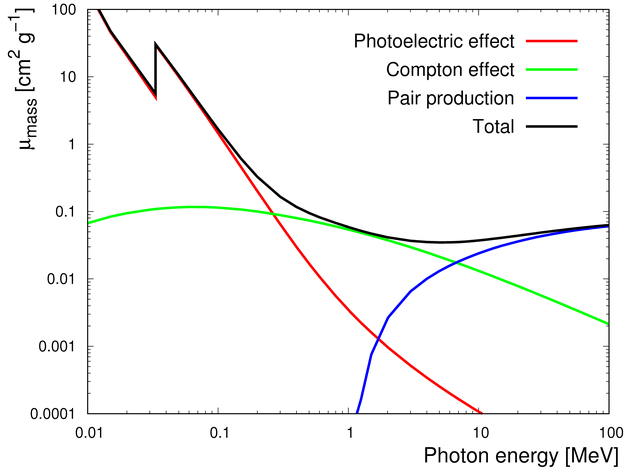
\includegraphics[scale=0.5]{pictures/extinction.png}
    \caption{Influence of the photoelectric effect, Compton scattering 
    and pair production on the extinction coefficient as a function of 
    energy \cite{LNT}.}
    \label{fig:extinction}
\end{figure}

\subsection{Function of a Semiconductor Detector}
\noindent
A semiconductor is a material with a valence and conduction band 
separated by a small band gap. At low temperatures, the valence 
band is fully occupied with electrons, while the conduction band 
remains empty. At higher temperatures, electrons can transition to 
the conduction band, leaving a hole in the valence band.

\noindent
Additionally, the semiconductor can be doped with atoms that 
introduce more or fewer valence electrons than the semiconductor. 
If the doping atom has fewer valence electrons, it creates an 
additional hole, resulting in a positively (p) doped material. 
Conversely, if the doping atom introduces more electrons, it leads 
to a negatively (n) doped material.

\noindent
A semiconductor detector essentially functions as a diode, where n 
and p doped regions border each other. The interface between these 
regions has fewer charge carriers due to recombination between the 
carriers from the n and p doped zones, creating a depletion zone. 
Recombination continues until the electric field of the remaining 
charges establishes equilibrium. The extent of the depletion zone 
can be expanded by applying an electric field.

\noindent
When a $\gamma$ photon is incident, it generates a high-energy 
electron through a process described in Section \ref{sec:process}. 
This energetic electron imparts its energy to other electrons in 
the semiconductor, causing them to jump from the valence to the 
conduction band. Consequently, a $\gamma$ photon creates multiple 
electrons and holes within the depletion zone. The electric field 
separates these charge carriers before they can recombine. The 
resulting charge pulse constitutes the measured signal. Thus the signal 
intensity increases with the energy of the incoming $\gamma$ photon.

\noindent
Figure \ref{fig:detector} depicts the schematic structure of a 
semiconductor detector.

\begin{figure}
    \centering
    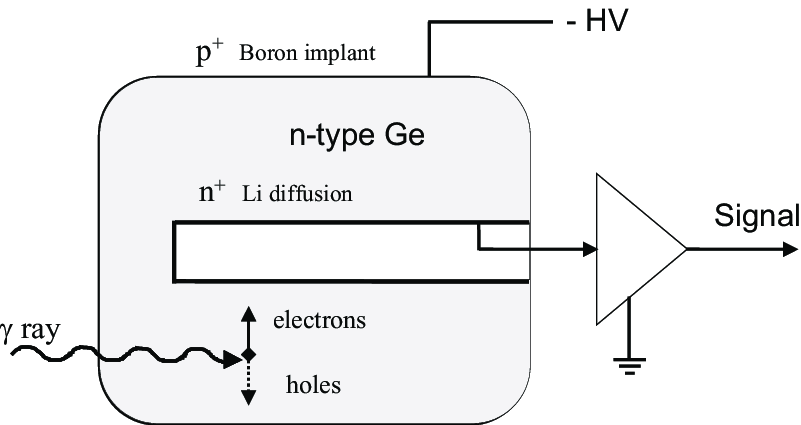
\includegraphics[scale=0.4]{pictures/detector.png}
    \caption{Schematic illustration of a germanium detector \cite{detector}.}
    \label{fig:detector}
\end{figure}

\subsection{Expected Spectrum of a Monochromatic γ Source}
The number of counts $N$ measured with a germanium detector, when a small 
$\gamma$ source is placed next to it, depends on the emission probability 
$P$ of the source, the activity $A$, the distance between the source and 
the detector (thus the solid angle component $\Omega$), and the time $t$. 
It is given by
\begin{equation}
    N_\text{theory} =  P \cdot \frac{\Omega}{4 \pi} \cdot A \cdot t.
\end{equation}

\noindent
If the source is monochromatic, meaning that all $\gamma$ photons have 
the same energy, the spectrum of the number of counts in dependence on 
the energy exhibits distinct peaks. Figure \ref{fig:spectrum} illustrates 
the expected spectrum of a monochromatic source, consisting of the 
photopeak, the Compton edge, and a backscattering peak in the Compton 
continuum. 

\noindent
The photopeak occurs at the energy of the $\gamma$ photon, as the entire 
energy of the photon is absorbed in the photoeffect. Below the photopeak 
lies the Compton continuum, with its maximum at the Compton edge where the 
scattering angle is $\theta=\pi$. Lower energies correspond to other 
scattering angles. Within the Compton continuum lies the backscattering 
peak, resulting from gammas undergoing Compton scattering outside the 
detector but backscattering into the detector before being fully absorbed.
The effect of pair production is not relevant for the sources used in this 
experiment.
\begin{figure}
    \centering
    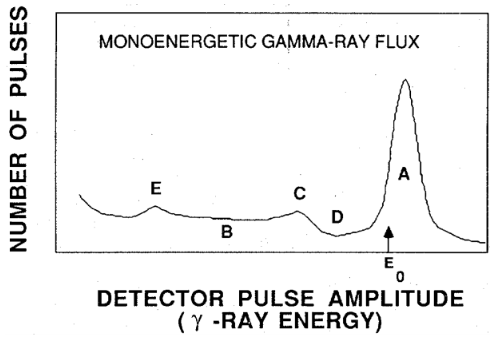
\includegraphics[scale=0.6]{pictures/spectrum.png}
    \caption{Spectrum of a monochromatic $\gamma$ source with the 
    photopeak (A), the Compton continuum (B), the Compton edge (C), 
    and the backscattering peak (E) \cite{Smith1997GammaRayD}.}
    \label{fig:spectrum}
\end{figure}